
\section{Metoda mapowania liniowego przy pomocy rozwinięcia w szereg Taylora}
\label{sec:Taylor}
Prezentowana w poniższej sekcji metoda kompensacji dyspersji została w artykule []\textcolor{red}{referenacja do yuanliu}
\subsection{Podstawy teoretyczne}
Po wzbudzeniu badanego pręta odpowiednim sygnałem wejściowym możliwe jest aby przełączył się on w tryb obioru sygnału i nasłuchiwał nadejścia odpowiedzi układu. W takim wypadku odpowiedź jaką uzyskamy będzie sumą odpowiedzi ze wszystkich odbić, od końca pręta oraz ewentualnych uszkodzeń.  Proponowana w tym rozdziale metoda opiera sie na założeniu, że w badanym obiekce propaguje jedna wybrana postać drgań. Jej celem jest kompensacja powstałej dyspersji, tak aby sygnały z różnych punktów odbicia nie nachodziły na siebie i była możliwa ich interpretacja w celu ustalenia ilości punktów odbicia oraz oszacowania ich odegłości od miejsca wzbudzenia na podstawie znajomości prędkości grupowej fali. Przy tak sformułowanych założeniach, sygnał otrzymany w odbiorniku można przedstawić wzorem:
\begin{equation}
g(t) = \sum\limits_{n=1}{N}f_n(r_n,t)=\frac{1}{2\pi}\int _{-\infty}^{\infty}F(\omega)\sum\limits_{n=1}^{N}(A_n(\omega)e^{-ikr_n})e^{i\omega t} d\omega \label{eq:g(t)_taylor}
\end{equation}
Gdzie:

$N$ - całkowita liczba ścieżek propagacji sygnału (liczba punktów odbicia)

$r_n$ - długość n-tej ścieżki propagacji

$A_n$ - współczynnik odbicia n-tego punktu odbicia.

Widmo częstotliwości takiego sygnału $G(\omega)$  możemy obliczyć przy pomocy transformaty Fouriera i zapisać wzorem:
\begin{equation}
G(\omega) = F(\omega)\sum\limits_{n=1}^{N}(A_n(\omega)e^{-ikr_n} \label{eq:G(omega)_taylor}
\end{equation}

Jak wiadomo, dyspersja zależy od kształtu krzywej dyspersji, $k = K(\omega)$. Jeśli więc $K(\omega)$ jest funkcją kwadratową lub wyższego rzędu względem $\omega$, to $G(\omega)$ reprezentuje widmo częstotliwości rozproszonych pakietów fal. Jeśli natomiast zależność $K(\omega)$ byłoby funkcją liniową, zjawisko dyspersji nie występowałoby, a $G(\omega)$ reprezentowałoby widmo częstotliwości sygnału, który nie uległ dyspersji. 
Wybraną krzywą dyspersji można przybliżyć przy pomocy rozwinięcia w szereg Taylora:
\begin{equation}
k = K(\omega) - k_0+k_1(\omega - \omega _0) + k_2(\omega - \omega _0^2)+... \label{eq:szereg_k}
\end{equation}

Gdzie:

$k_0 = \frac{\omega _0}{c_p}$

$k_1 = \frac{dk}{d\omega}|_{\omega = \omega_0}$

$k_2 = \frac{1}{2}\frac{d^2k}{d\omega ^2}|_{\omega = \omega _0}$

$c_p$ - prędkość fazowa

Wynika z tego, iż dyspersję sygnału można usunąć usuwając jej nieliniowy składnik, poprzez zastąpienie oryginalnej zależności $K(\omega)$ liniowym przybliżeniem tej funkcji. Zastosowanie takiego zabiegu sprawi, iż sygnał w dziedzinie czasu będzie postrzegany jako skompensowany do postaci niedyspersyjnej, a prędkość grupowa obliczona z liniowego przybliżenia krzywej dyspersji może zostać wykorzystana do określenia długości ścieżek propagacji wynikających z kolejnych odbić. 

W szczególnym przypadku, w którym mamy do czynienia z pojedyńczą ścieżką propagacji ($N=1$) i odległość między nadajnikiem a punktem odbicia jest znana, można usunąć dyspersję poprzez wyeliminowanie wyrażenia kwadratowego w $K(\omega)$. Matematycznie można to zrobić przy pomocy wzoru:
\begin{equation}
 \widetilde{G}(\omega)=(F(\omega)A_1(\omega)e^{-ikr_1})e^{ik_2(\omega -\omega _0)^2r_1}
\end{equation}

Gdzie $\widetilde{G}(\omega)$ jest zmodyfikowanym widmem częstotliwości, a $r_1$ jest odległością między nadajnikiem i odbiornikiem. Sygnał skompensowany w dziedzinie czasu można natychmiast uzyskać poprzez odwrotną transformatę Fouriera. Ponieważ jednak zazwyczaj długość ścieżki propagacji sygnału nie jest znana, a sygnał może składać się z wielu odbić, między innymi od uszkodzeń ($N>1$) usuwanie dyspersji przy pomocy powyższego wzoru byłoby niepraktyczne. 

Rysunek \ref{fig:krzywa_taylorem} obrazuje przykład krzywej dyspersji, trybu $A_0$, płyty aluminiowej o grubości 3,175 mm. Linia ciągła pokazuje zależności $K(\omega)$ uzyskaną metodami komputerowymi, natomiast linia przerywana kropkowana wskazuje z rozwinięcie szeregu Taylora pierwszego rzędu, a linia przerywana rozszerzenie szeregu Taylora drugiego rzędu w odniesieniu do centralnej częsości kątowej ($\omega _0 = 2\pi *50 kHz$)

\begin{figure}[h]
\centering
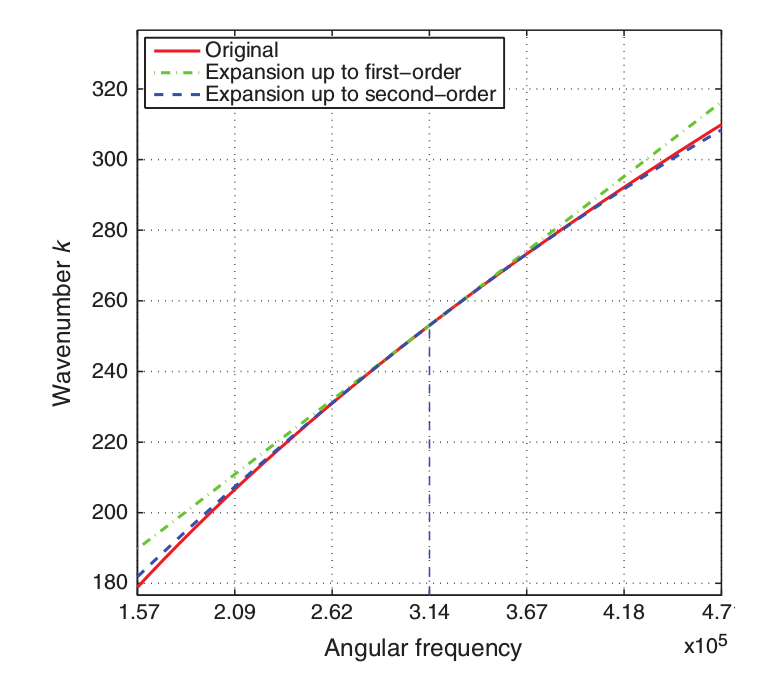
\includegraphics[width=14cm]{Zdjecia/4/buba}
\caption{Przykładowe porównanie oryginalnej krzywej oraz jej przybliżeń przy pomocy rozwinięcia w szereg Taylora}
\label{fig:krzywa_taylorem}
\end{figure}

Łatwo zauważyć, że po pierwsze, rozszerzenie drugiego rzędu daje bardzo dobrze przybliżenie pierwotnego kształtu krzywej, po drugie, $K(\omega)$ jest monotoniczną funkcją $\omega$ w oroczeniu $\omega _0$. 

Równanie \ref{eq:G(omega)_taylor} można zapisać w postacji złożenia funkcji:
\begin{equation}
G(\omega) = G(k)\circ K(\omega)
\end{equation}

Gdzie $\circ$ jest operatorem składania funkcji. $G(k)$ jest niejawną funkcją k z równania \ref{eq:G(omega)_taylor}. Zamieniając $K(\omega)$ na $K_{lin}(\omega)$ będące aproksymacją $K(\omega)$ pierwszego rzędu w punkcie $\omega _0$, gdzie $\omega _0$ oznacza częstotliwość o najwyższej energii, można wyprowadzić zmodyfikowane widmo częstotliwości:
\begin{equation}
\widetilde{G}(\omega) = G(k)\circ K_{lin}(\omega)
\end{equation}

Ponieważ $G(\omega)$ jest znane oraz znana jest analizowana krzywa dyspersji, znane jest również $G(k)$, obliczając przybliżenie liniowe $K_{lin}(\omega)$ można w prosty psosób obliczyć $\widetilde{G}(\omega)$, poprzez interpolację odpowiednich wartości. Opisana metoda może być określana mianem mapowania liniowego. W jej efekcie uzyskane zostaje nowe widmo częstotliwości $\widetilde{G}(\omega)$. Po mapowaniu widmo amplitudy pozostaje bez zmian, natomiast widmo fa